\documentclass[landscape, a4paper]{article}
\usepackage[margin=0cm,top=0.4cm,bottom=0.4cm,left=0.4cm,right=0.4cm]{geometry}
% \usepackage[showframe,margin=0cm,top=0.5cm,bottom=0.5cm,left=0.5cm,right=0.5cm]{geometry}
\usepackage[export]{adjustbox}
\usepackage{ipsum}
\usepackage{xcolor}
\usepackage{caption}
\usepackage{tabularray}
\usepackage{csquotes}
\usepackage{titlesec}
\usepackage{etoolbox} % Add this to your preamble
\usepackage[parfill]{parskip}

\newtoggle{isEnglish}
% \toggletrue{isEnglish}
\togglefalse{isEnglish}

\captionsetup{labelformat=empty, justification=centering, font={color=PrimaryColor}}

\definecolor{PrimaryColor}{HTML}{DD6503}
\definecolor{PrimaryColorDimmed}{HTML}{f1c197}
\colorlet{BoxColor}{gray!10!white}
\newcommand\alert[1]{\textcolor{PrimaryColor}{\textbf{#1}}}

\usepackage{amssymb} % For \blacktriangleright and other symbols

\renewcommand{\labelitemi}{$\textcolor{PrimaryColor}{\bullet}$}
\renewcommand{\labelitemii}{$\textcolor{PrimaryColor}{\blacktriangleright}$}
\renewcommand{\labelitemiii}{$\textcolor{PrimaryColor}{\blacksquare}$}

\renewcommand{\labelenumi}{\textbf{\textcolor{PrimaryColor}{\theenumi.}}}
\renewcommand{\labelenumii}{\textbf{\textcolor{PrimaryColor}{\theenumii.}}}
\renewcommand{\labelenumiii}{\textbf{\textcolor{PrimaryColor}{\theenumiii.}}}

\titleformat{\section}
{\color{PrimaryColor}\normalfont\large\bfseries}
{\thesection}{0.5cm}{}
\titlespacing{\section}{0cm}{0.2cm}{0.2cm}

\titleformat{\subsection}
{\color{PrimaryColor}\normalfont\normalsize\bfseries}
{\thesubsection}{0.5cm}{}
\titlespacing{\subsection}{0cm}{0.1cm}{0.1cm}

% \titleformat{\subsubsection}
% {\color{PrimaryColor}\normalfont\normalsize\bfseries}
% {\thesubsection}{0.5cm}{}
% \titlespacing{\subsubsection}{0cm}{0.1cm}{0.1cm}

\begin{document}
\noindent
\centering
\footnotesize
\begin{minipage}[t]{0.31\textwidth}
	\vspace{0.5cm}
	\setlength{\parskip}{0.25cm}

	\textcolor{PrimaryColor}{
		\rule{\linewidth}{0.5mm}
		\vspace{-0.1cm}
		\begin{center}
			\large
			\textsc{California Roll (1 Roll - 8 pieces)}
		\end{center}
		\rule{\linewidth}{0.5mm}
	}

	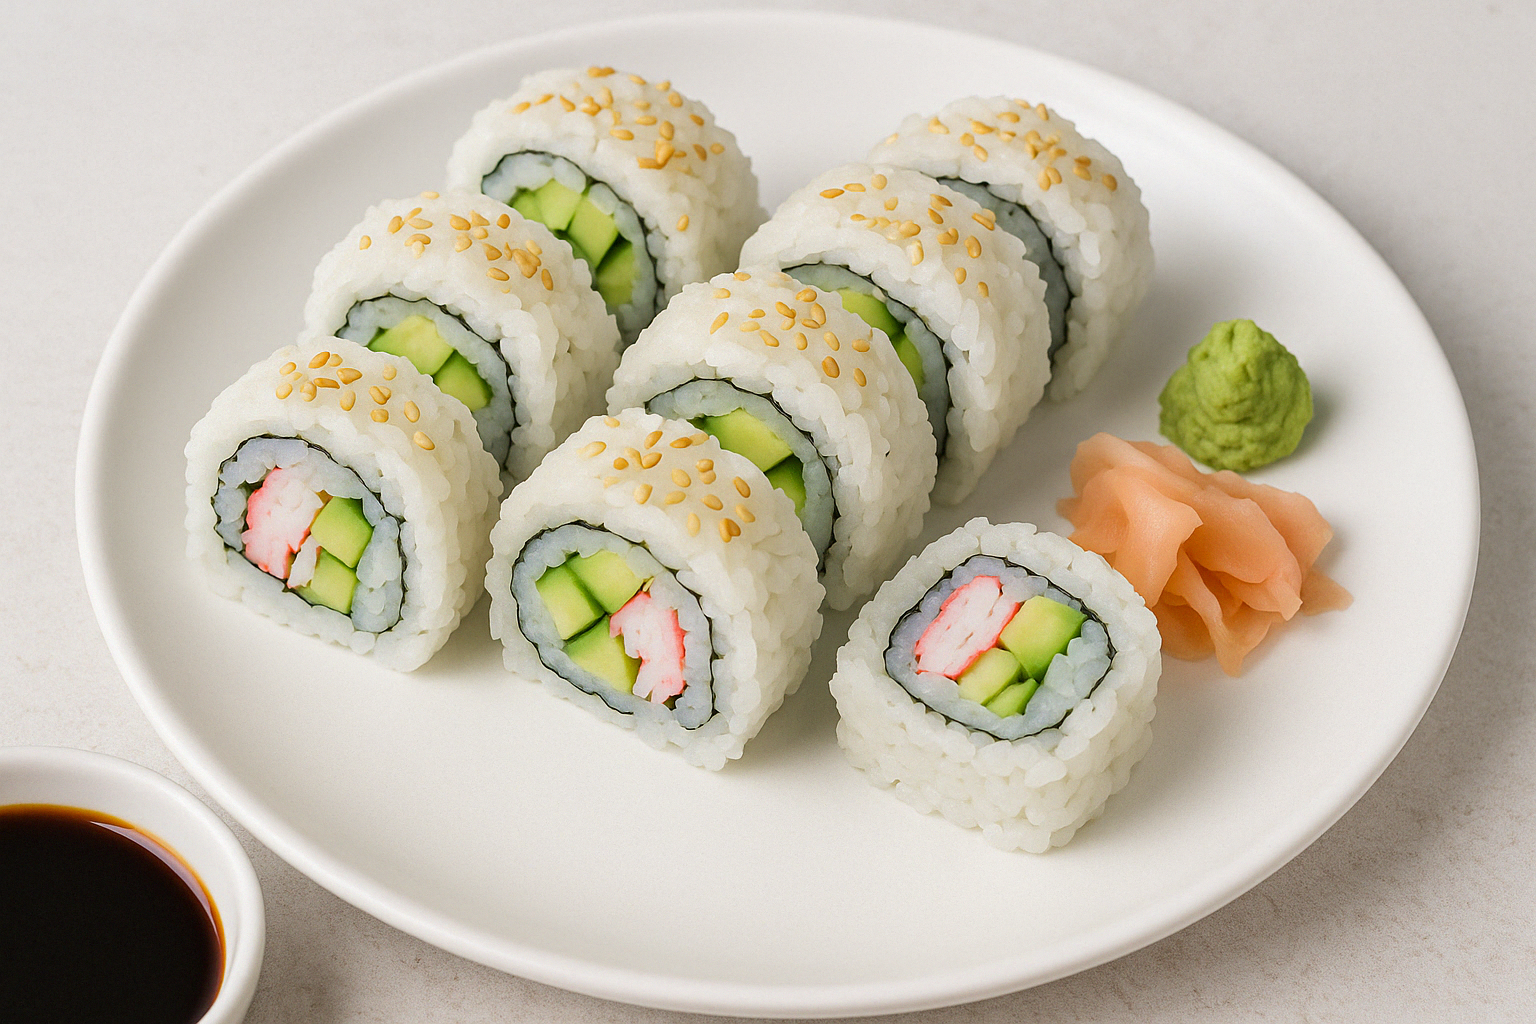
\includegraphics[width=\linewidth]{./figures/california_rolls.png}

	\section*{Ingredients}

	\resizebox{\textwidth}{!}{
		\begin{tblr}{
				width = \textwidth,
				cells = {bg=BoxColor},
				row{1} = {PrimaryColor,c,fg=white},
				row{2} = {PrimaryColorDimmed},
				row{8} = {PrimaryColorDimmed},
				row{16} = {PrimaryColorDimmed},
				row{20} = {PrimaryColorDimmed},
				cell{2}{1} = {c=2}{},
				cell{8}{1} = {c=2}{},
				cell{16-19}{1} = {c=2}{},
			}
			\textbf{Ingredient}                               & \textbf{Amount}                        \\
			For the sushi rice:                               &                                        \\
			Sushi rice                                        & 100g                                   \\
			Water                                             & 120ml                                  \\
			Rice vinegar                                      & 15ml                                   \\
			Sugar                                             & 7g                                     \\
			Salt                                              & 2g                                     \\
			For the roll:                                     &                                        \\
			Nori sheet (half sheet):                          & 1 piece ($\sim$18x10 cm)               \\
			Imitation crab stick (surimi):                    & 30 g (2 sticks or shredded equivalent) \\
			Cucumber (seeded):                                & 15 g (cut into matchsticks)            \\
			Ripe avocado:                                     & 20 g (cut into thin strips)            \\
			Toasted white sesame seeds:                       & 1 tsp (3 g)                            \\
      Mayonnaise (preferably Japanese mayo like Kewpie) & 10 g (about 2 tsp) \\

      Sriracha or another chili sauce (adjust to taste) & 2–3 g (½ tsp) \\

			For serving:                                      &                                        \\
			Soy sauce                                         &                                        \\
			Pickled ginger                                    &                                        \\
			Wasabi                                            &                                        \\
			Equipment Needed:                                 &                                        \\
			Bamboo sushi mat (makisu) wrapped in plastic wrap &                                        \\
			Sharp knife (preferably moistened for cutting)    &                                        \\
			Bowl of water (to prevent sticking)               &                                        \\
		\end{tblr}
	}
\end{minipage}%
\hfill%
\vrule width 0.01cm
\hfill%
\begin{minipage}[t]{0.31\textwidth}
	\vspace{0cm}
	\setlength{\parskip}{0.25cm}

	\section*{Instructions}
	\vspace{0.25cm}

	\subsection*{1. Prepare the Sushi Rice (40–60 mins)}
	\vspace{0.25cm}
	\begin{enumerate}
		\item \alert{Rinse the rice:} Rinse 100 g sushi rice under cold water until the water runs clear. Drain and let rest for 10 minutes.
		\item \alert{Cook the rice:} Combine the rice with 120 ml water in a pot. Bring to a boil, then simmer on low heat for 10 minutes. Let it steam (covered) for an additional 10 minutes.
		\item \alert{Season the rice:} Gently heat 15 ml rice vinegar, 7 g sugar, and 2 g salt until dissolved. Fold into the cooked rice and let cool to body temperature.
	\end{enumerate}

	\subsection*{2. Prepare the Fillings (5–10 mins)}
	\begin{itemize}
		\item Peel and seed the cucumber, then slice into thin matchsticks (approx.\ 5 mm wide, 8 cm long).
		\item Cut avocado into thin strips.
		\item Shred or slice imitation crab if necessary.
    \item Mix 10 g mayonnaise with 2–3 g sriracha in a small bowl. Stir until smooth. For spicy mayo 
	\end{itemize}

	\subsection*{3. Assemble the Roll (10 mins)}
	\begin{enumerate}
		\item Place plastic-wrapped bamboo mat on a flat surface.
		\item Place half a nori sheet (rough side up) on the mat.
		\item Wet fingers and evenly spread 90–100 g of sushi rice on the nori.
		\item Sprinkle with 3 g sesame seeds.
		\item Carefully flip the nori so rice faces down.
		\item Arrange 30 g imitation crab, 15 g cucumber, and 20 g avocado in a horizontal line, 2–3 cm from the near edge. Drizzle or spread about 1 tsp (5 g) of the spicy mayo directly over the fillings.
		\item Roll the mat forward gently but tightly to form a cylinder.
	\end{enumerate}

	\subsection*{4. Cut the Roll (2–3 mins)}
	\begin{itemize}
		\item Dip a sharp knife in water-vinegar mix.
		\item Cut the roll in half, then cut each half into 4 even pieces.
	\end{itemize}

	\subsection*{5. Serve}
	\begin{itemize}
		\item Arrange the 8 pieces cut-side up.
		\item Serve with soy sauce, wasabi, and pickled ginger if desired.
	\end{itemize}

	% \section*{Tips}
	% \begin{itemize}
	% 	\item Don’t overload the roll, use thin layers
	% 	\item Keep hands damp, not wet, when handling rice
	% 	\item Use plastic wrap over the bamboo mat for easier rolling.
	% \end{itemize}

	% 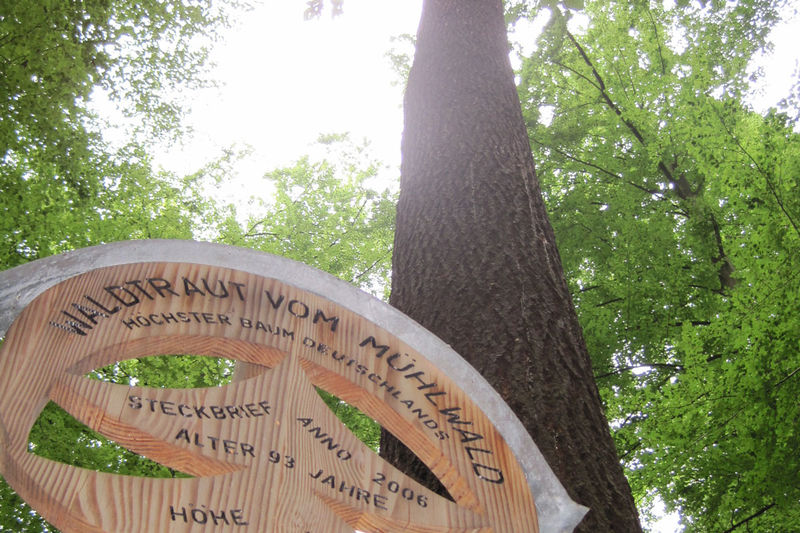
\includegraphics[width=\linewidth]{./figures/waldraud.png}
	%  \captionof{figure}{\iftoggle{isEnglish}{Waldtraut of the Mühlwald, the tallest officially measured tree in Germany}{Waldtraut vom Mühlwald, höchster amtlich vermessener Baum Deutschlands}}
	% \setlength{\parskip}{0.25cm}

\end{minipage}%
\hfill\color{white}%
\vrule width 0.01cm
\hfill\color{black}%
\begin{minipage}[t]{0.31\textwidth}
	\vspace{0.5cm}
	\setlength{\parskip}{0.25cm}

	\textcolor{PrimaryColor}{
		\rule{\linewidth}{0.5mm}
		\vspace{-0.1cm}
		\begin{center}
			\large
			\textsc{History of Sushi}
		\end{center}
		\rule{\linewidth}{0.5mm}
	}

	The \alert{word sushi} comes from the Japanese phrase \enquote{su} (vinegar) and \enquote{shi} (rice), referring to vinegared rice that is combined with ingredients like raw or cooked fish, vegetables, or egg.

	Sushi originated over a \alert{thousand years ago} in Southeast Asia as a method of preserving fish by fermenting it with rice. This early form, called narezushi, allowed people to store fish for months. When it reached Japan around the 8th century, it gradually evolved. Eventually, the Japanese started eating the rice along with the fish, shortening the fermentation process.

	By the \alert{Edo period} (1603–1868), a faster, fresher form of sushi emerged: edomae zushi, named after Edo (modern-day Tokyo). This style featured raw or cured fish atop small rice balls and was sold as street food. It became the prototype for today’s nigiri sushi.

	When sushi began to evolve from narezushi (fermented fish) to edomae sushi, chefs began experimenting with portable forms of the dish. \alert{Rolled sushi} (maki-zushi) became popular as it was easy to eat on the go. Nori sheets were the perfect tool for this: they held everything together and added a crisp, ocean-like flavor that complemented the rice and fish.

	\alert{Nori} has been eaten in Japan for over a thousand years, but it wasn't always in sheet form. Originally, it was scraped from rocks in tidal areas and sold as a paste (nori-tsukudani). Around the 1700s, during the Edo period, Japanese food producers developed a method to dry and shape seaweed into paper-like sheets—inspired by traditional paper-making techniques. This innovation made it much easier to store, handle, and use nori in new ways.

	Western sushi, especially in places like the U.S., has taken creative liberties with traditional forms. Rolls like the \alert{California Roll} (with imitation crab, avocado, and cucumber) were created in Los Angeles in the 1960s, likely by chef Ichiro Mashita to appeal to Western tastes and avoid raw fish (replacing raw tuna with avocado and imitation crab called surimi). The \alert{Dragon Roll} is another modern creation, usually filled with eel and cucumber and topped with avocado to resemble dragon scales.

	\alert{Traditional Japanese sushi} emphasizes balance, seasonality, and simplicity. Raw fish is served in delicate slices, highlighting the freshness and natural flavor. Rice is subtly seasoned, and garnishes like wasabi, soy sauce, or pickled ginger are used sparingly.

	\alert{Western sushi}, particularly in the U.S., Canada, and Europe, tends to be more fusion-oriented. It includes non-traditional ingredients like avocado, cream cheese, spicy mayonnaise, and fried elements. Rolls are often large, richly flavored, and visually elaborate. This adaptation helped sushi become more accessible to Western palates.

\end{minipage}%

\newpage

\begin{minipage}[t]{0.31\textwidth}
	\setlength{\parskip}{0.25cm}
	\vspace{0.5cm}

	\textcolor{PrimaryColor}{
		\rule{\linewidth}{0.5mm}
		\vspace{-0.1cm}
		\begin{center}
			\large
			\textsc{Futomaki Sushi Roll (1 Roll – 8 Pieces)}
		\end{center}
		\rule{\linewidth}{0.5mm}
	}

	% \includegraphics[width=\linewidth]{./figures/futomaki_sushi_roll.png}
	% \includegraphics[width=\linewidth]{./figures/futomaki_sushi_roll_on_plate.png}
	% \includegraphics[width=\linewidth]{./figures/futomaki_sushi_roll_2.png} 
	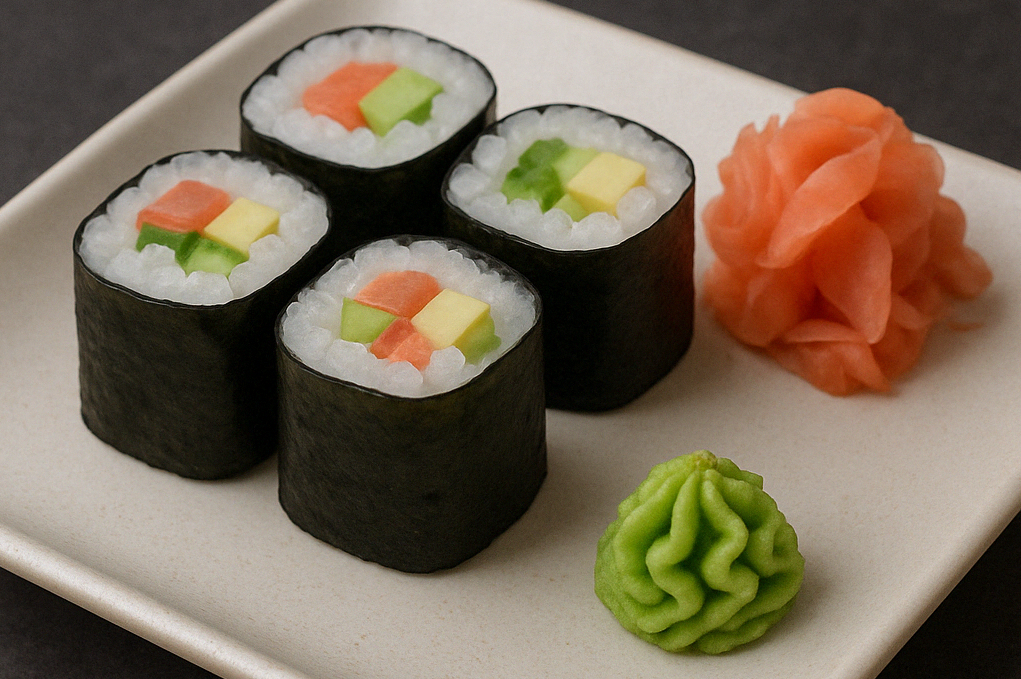
\includegraphics[width=\linewidth]{./figures/futomaki_sushi.png}

	\section*{Ingredients}

	\resizebox{\textwidth}{!}{
		\begin{tblr}{
				width = \textwidth,
				cells = {bg=BoxColor},
				row{1} = {PrimaryColor,c,fg=white},
				row{2} = {PrimaryColorDimmed},
				row{8} = {PrimaryColorDimmed},
				row{11} = {PrimaryColorDimmed},
				row{15} = {PrimaryColorDimmed},
				% row{14} = {PrimaryColorDimmed},
				cell{2}{1} = {c=2}{},
				cell{8}{1} = {c=2}{},
				cell{10-17}{1} = {c=2}{},
			}
			\textbf{Ingredient}                               & \textbf{Amount}          \\
			For the sushi rice:                               &                          \\
			Sushi rice                                        & 90g                      \\
			Water                                             & 120ml                    \\
			Rice vinegar                                      & 15ml                     \\
			Sugar                                             & 7g                       \\
			Salt                                              & 2g                       \\
			For the roll:                                     &                          \\
			Nori sheet (half sheet):                          & 1 piece ($\sim$18x10 cm) \\
			See list of possible ingridients on right         &                          \\
			For serving:                                      &                          \\
			Soy sauce                                         &                          \\
			Pickled ginger                                    &                          \\
			Wasabi                                            &                          \\
			Equipment Needed:                                 &                          \\
			Bamboo sushi mat (makisu) wrapped in plastic wrap &                          \\
			Sharp knife (preferably moistened for cutting)    &                          \\
			Bowl of water (to prevent sticking)               &                          \\
		\end{tblr}
	}

\end{minipage}%
\hfill%
\vrule width 0.01cm
\hfill%
\begin{minipage}[t]{0.31\textwidth}
	\vspace{0cm}
	\setlength{\parskip}{0.25cm}

	\section*{Instructions}
	\vspace{0.25cm}

	\subsection*{1. Prepare the Sushi Rice}
	\vspace{0.25cm}
	\begin{enumerate}
		\item \alert{Rinse the rice}: Rinse the rice under cold water 3--4 times until the water runs clear. Let it drain in a sieve for 15 minutes.
		\item \alert{Cook the rice}: Combine rice with \(120\,\mathrm{ml}\) water in a pot. Soak for 30 minutes, then bring to a boil. Reduce heat, cover, and cook on low for 13 minutes. Let steam for another 10 minutes off the heat.
		\item \alert{Season the rice}: Mix \(15\,\mathrm{ml}\) vinegar, \(7\,\mathrm{g}\) sugar, and \(2\,\mathrm{g}\) salt. Gently fold into the cooked rice using a cutting motion. Cool to room temperature while fanning.
	\end{enumerate}

	% \subsection*{2. Prepare Tamagoyaki (Optional)}
	\subsection*{2. Prepare Fillings}
	\begin{itemize}
		\item Beat 2 eggs with \(5\,\mathrm{ml}\) soy sauce, \(5\,\mathrm{g}\) sugar, and a pinch of salt. Cook in a non-stick pan in layers, rolling each layer. Let cool and cut a strip about \(15\,\mathrm{cm} \times 3\,\mathrm{cm} \times 1\,\mathrm{cm}\).
		% \end{enumerate}

		% \subsection*{3. Prepare Other Fillings}
		% \begin{itemize}
		% \item \alert{Kanpyo}: Soak 30 minutes, then simmer in water with soy sauce and sugar.
		% \item \alert{Shiitake}: Rehydrate and simmer in \(100\,\mathrm{ml}\) water with \(5\,\mathrm{ml}\) soy sauce and \(5\,\mathrm{g}\) sugar until liquid reduces.
		% \item \alert{Carrot}: Blanch for 1 minute or lightly pickle in vinegar.
	\end{itemize}

	\subsection*{3. Assemble the Futomaki Roll}
	\begin{enumerate}
		\item Place the bamboo mat on a flat surface. Lay the nori sheet shiny side down.
		\item Spread about \(90\,\mathrm{g}\) of rice evenly on the nori, leaving a \(2\,\mathrm{cm}\) border at the top.
		\item Arrange the fillings horizontally across the center.
		\item Roll the sushi tightly using the mat, applying gentle pressure to shape a firm roll.
		% \item Wet a sharp knife and slice into 8 equal pieces.
	\end{enumerate}

	\subsection*{4. Cut the Roll (2–3 mins)}
	\begin{itemize}
		\item Dip a sharp knife in water-vinegar mix.
		\item Cut the roll in half, then cut each half into 4 even pieces.
	\end{itemize}

	\subsection*{5. Serve}
	\begin{itemize}
		\item Arrange the 8 pieces cut-side up.
		\item Serve with soy sauce, wasabi, and pickled ginger if desired.
	\end{itemize}

\end{minipage}%
\hfill%
\vrule width 0.01cm
\hfill%
\begin{minipage}[t]{0.31\textwidth}
	\vspace{0.5cm}
	\setlength{\parskip}{0.25cm}

	\textcolor{PrimaryColor}{
		\rule{\linewidth}{0.5mm}
		\vspace{-0.1cm}
		\begin{center}
			\large
			\textsc{Types of Sushi}
		\end{center}
		\rule{\linewidth}{0.5mm}
	}

	\begin{itemize}
		\item \alert{Nigiri:}
		The word \textit{nigiri} comes from the Japanese verb \textit{nigiru}, meaning \enquote{to grasp} or to \enquote{squeeze with the hand}. It refers to how the sushi is hand-pressed into a small oval shape.
		A piece of sushi rice is formed by hand and topped with a slice of fish, seafood, or egg. Some nigiri is lightly brushed with soy sauce or wasabi. The topping can be raw (like tuna or salmon), cooked (such as shrimp or eel), or marinated.

		\item \alert{Maki – Rolled Sushi:}
		\textit{Maki} comes from the verb \textit{maku}, which means \enquote{to roll}. Maki sushi is rolled using a bamboo mat (\textit{makisu}) and wrapped in seaweed (\textit{nori}). It is then cut into bite-sized pieces. Typically, it includes rice and one or more fillings such as fish, cucumber, or avocado.
		\begin{itemize}
			\item \alert{Hosomaki:}
			The word \textit{hosoi} means \enquote{thin}, and \textit{maki} means \enquote{roll}, so \textit{hosomaki} is a \enquote{thin roll}. It contains one simple filling like tuna (\textit{tekka maki}) or cucumber (\textit{kappa maki}), wrapped in nori with rice inside.

			\item \alert{Futomaki:}
			\textit{Futoi} means \enquote{fat} or \enquote{thick}, so \textit{futomaki} is a \enquote{thick roll}. It includes multiple colorful fillings, vegetables, cooked ingredients, and sometimes egg, creating a rich and decorative look.
		\end{itemize}

		\item \alert{Uramaki – Inside-out Roll:}
		\textit{Ura} means \enquote{reverse} or \enquote{inside-out}, so \textit{uramaki} is a \enquote{reverse roll}. This Western-invented style has the rice on the outside and nori hidden inside. Uramaki often includes sesame seeds, fish roe, or sauces on the outside, offering a more complex taste and visual appeal.
	\end{itemize}

	\textcolor{PrimaryColor}{
		\rule{\linewidth}{0.5mm}
		\vspace{-0.1cm}
		\begin{center}
			\large
			\textsc{Types of Filings}
		\end{center}
		\rule{\linewidth}{0.5mm}
	}

	\begin{minipage}[t]{0.48\textwidth}
		\begin{itemize}
			\item Tamagoyaki (Japanese omelette): 1 piece, about 30 g (instructions above)
      \item Tofu
      \item Grilled chicken (teriyaki or plain)
      \item Beef strips (shabu shabu-style or teriyaki beef)
      \item Cream cheese
      \item Tempura shrimp
      \item Surimi (paste from white fish processed and flavored to imitation crab)
		\end{itemize}
	\end{minipage}
	\hfill
	\begin{minipage}[t]{0.48\textwidth}
		\begin{itemize}
			\item Cucumber (julienned): 20 g
			\item Carrot (julienned, lightly blanched or pickled): 15 g
      % \item Kanpyo (dried gourd strips): 10 g (rehydrated) – optional
      % \item Shiitake mushrooms (sweet-simmered): 20 g
      \item Pickled daikon radish (takuan): 10 g
      \item Avocado (sliced): 30 g
      \item Mango
      \item Pineapple
      \item Jalapeño
      \item Sun-dried tomato
		\end{itemize}
	\end{minipage}

\end{minipage}%

\end{document}
